\section{Case Study}
An example of a real industrial \emph{product detection sorting system} will be shown.

\subsection{Product Detection Sorting System}
The product detection sorting system is mainly for product quality detecting, as well as sorting. The path delivery facility transmits the product to two conveyors by turns. Both the two conveyors have the \emph{read device} and \emph{write device}, respectively. The read device takes the \emph{info} from the product to check the quality of the product, and then write the detecting results mark to the product. The sorting section separates the produce by scanning the detecting mark on the product and decide to sort the product into the qualified area or disqualified area.


\subsection{Implement of System Model}
As introduced above, we will describe how to model the system using $IMCL$. The implement of the system model includes three parts:

\textbf{(1) Unifying the resources.} \ \emph{SENSOR} and \emph{DEVICE} are the two types of resource sets where the system can get physical information. The system can get the info from these sensors and control those devices.

\begin{equation*}
\footnotesize
    \begin{aligned}
       & \textbf{SENSOR: }  \{ \ pathSensor, \ sensor1, \ sensor2, \ sortSensor \ \}; \\
       & \textbf{DEVICE: }  \{ \ \emph{PATHSET}, \ \emph{SREAD}1, \ \emph{SWRITE}1, \ \emph{SREAD}2, \ \emph{SWRITE}2, \\
       & \ \ \ \ \ \ \ \ \ \ \ \ \ \ \ \ \emph{SCANNER}, \ \emph{SORTSET} \ \};
    \end{aligned}
\end{equation*}

\begin{figure}[!htb]
    \centering
        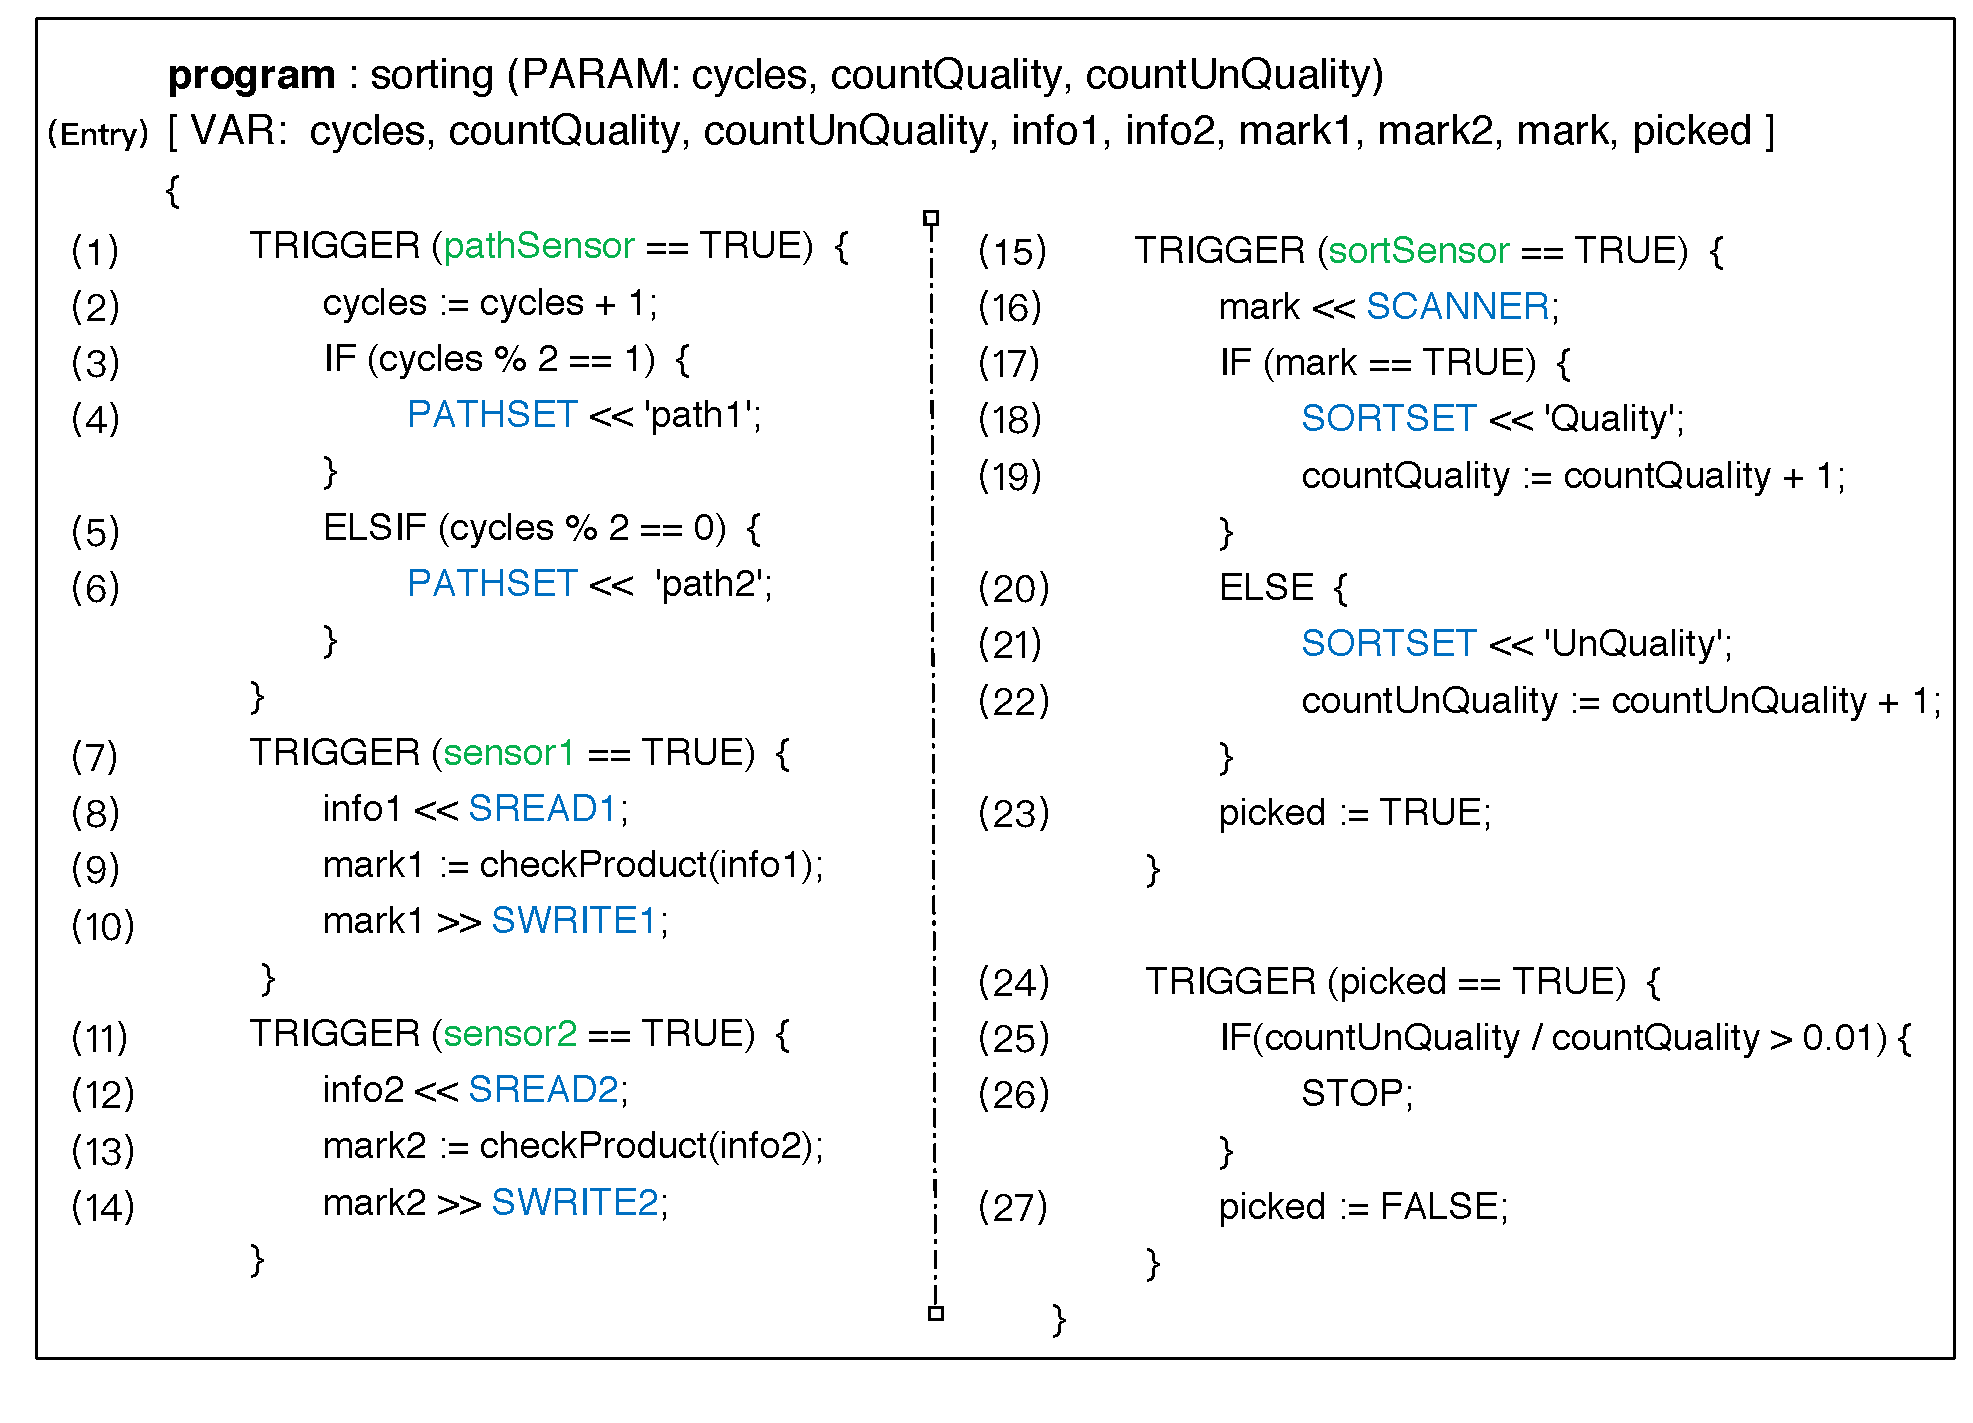
\includegraphics[height=2.5in, width=3.5in]{fig_IMCL_code}
    \caption{Modeling the system using IMCL}\label{fig_IMCL_code}
\end{figure}

\textbf{(2) Modeling the system.} \ Fig.\ref{fig_IMCL_code} is the \emph{product detection sorting system}. The model contains five event triggers. The first one is triggered when \emph{pathSensor} is true, and \emph{PATHSET} will take a product to the two conveyors. The second one is triggered when the \emph{sensor1} is true; then the \emph{SEAD1} reads the information from the product to check whether it is qualified or not, and then the \emph{SWRITE1} marks the checking result on the product and so does the third event trigger. The fourth one indicates that when the \emph{pathSensor} is true, then the sorting device will determine the sorting of the product by the inspection mark on the product scanned by \emph{SCANNER}. The fifth one indicates that the system checks the system after the \emph{pick} becomes real.

\textbf{(3) Defining resource constraints.} \ The constraints of the resources describe the ability of every \emph{CU}. For example, the computing unit $B_{cu}$ can control two resources \emph{pathSensor} and \emph{PATHSET} in this system model.
\begin{equation*}
\footnotesize
    \begin{aligned}
        \ \textbf{constraint : \ } & \textbf{$A_{cu}$} \ \{ \ \emph{SCANNER}, \ sortSensor, \ \emph{SWRITE}2 \ \};\\
        \ \textbf{constraint : \ } & \textbf{$B_{cu}$} \ \{ \ pathSensor, \ \emph{PATHSET} \ \};\\
        \ \textbf{constraint : \ } & \textbf{$C_{cu}$} \ \{ \ sensor1, \ sensor2, \ \emph{SREAD}2, \ \emph{PATHSET} \ \};\\
        \ \textbf{constraint : \ } & \textbf{$D_{cu}$} \ \{ \ \emph{SREAD}1, \ \emph{SWRITE}1, \ \emph{SORTSET} \ \};
    \end{aligned}
\end{equation*}

\subsection{Decomposition and Collaboration}

As shown in Fig.\ref{fig_IMCL_code}, there are 27 statements in the model that every statement is the minimum computational task level we want to decompose.
The Fig.\ref{fig_four_collaborated_program} shows that four \emph{CU}s are all have a set of statements corresponding to the minimum computational tasks in the original model.
For example, the $C_{cu}$ decomposed with the set $\{7,11,12\}$, means that the $C_{cu}$ can handle to statement 7, 11 and 12 in sorting system model.

\begin{figure}[!htb]
    \centering
        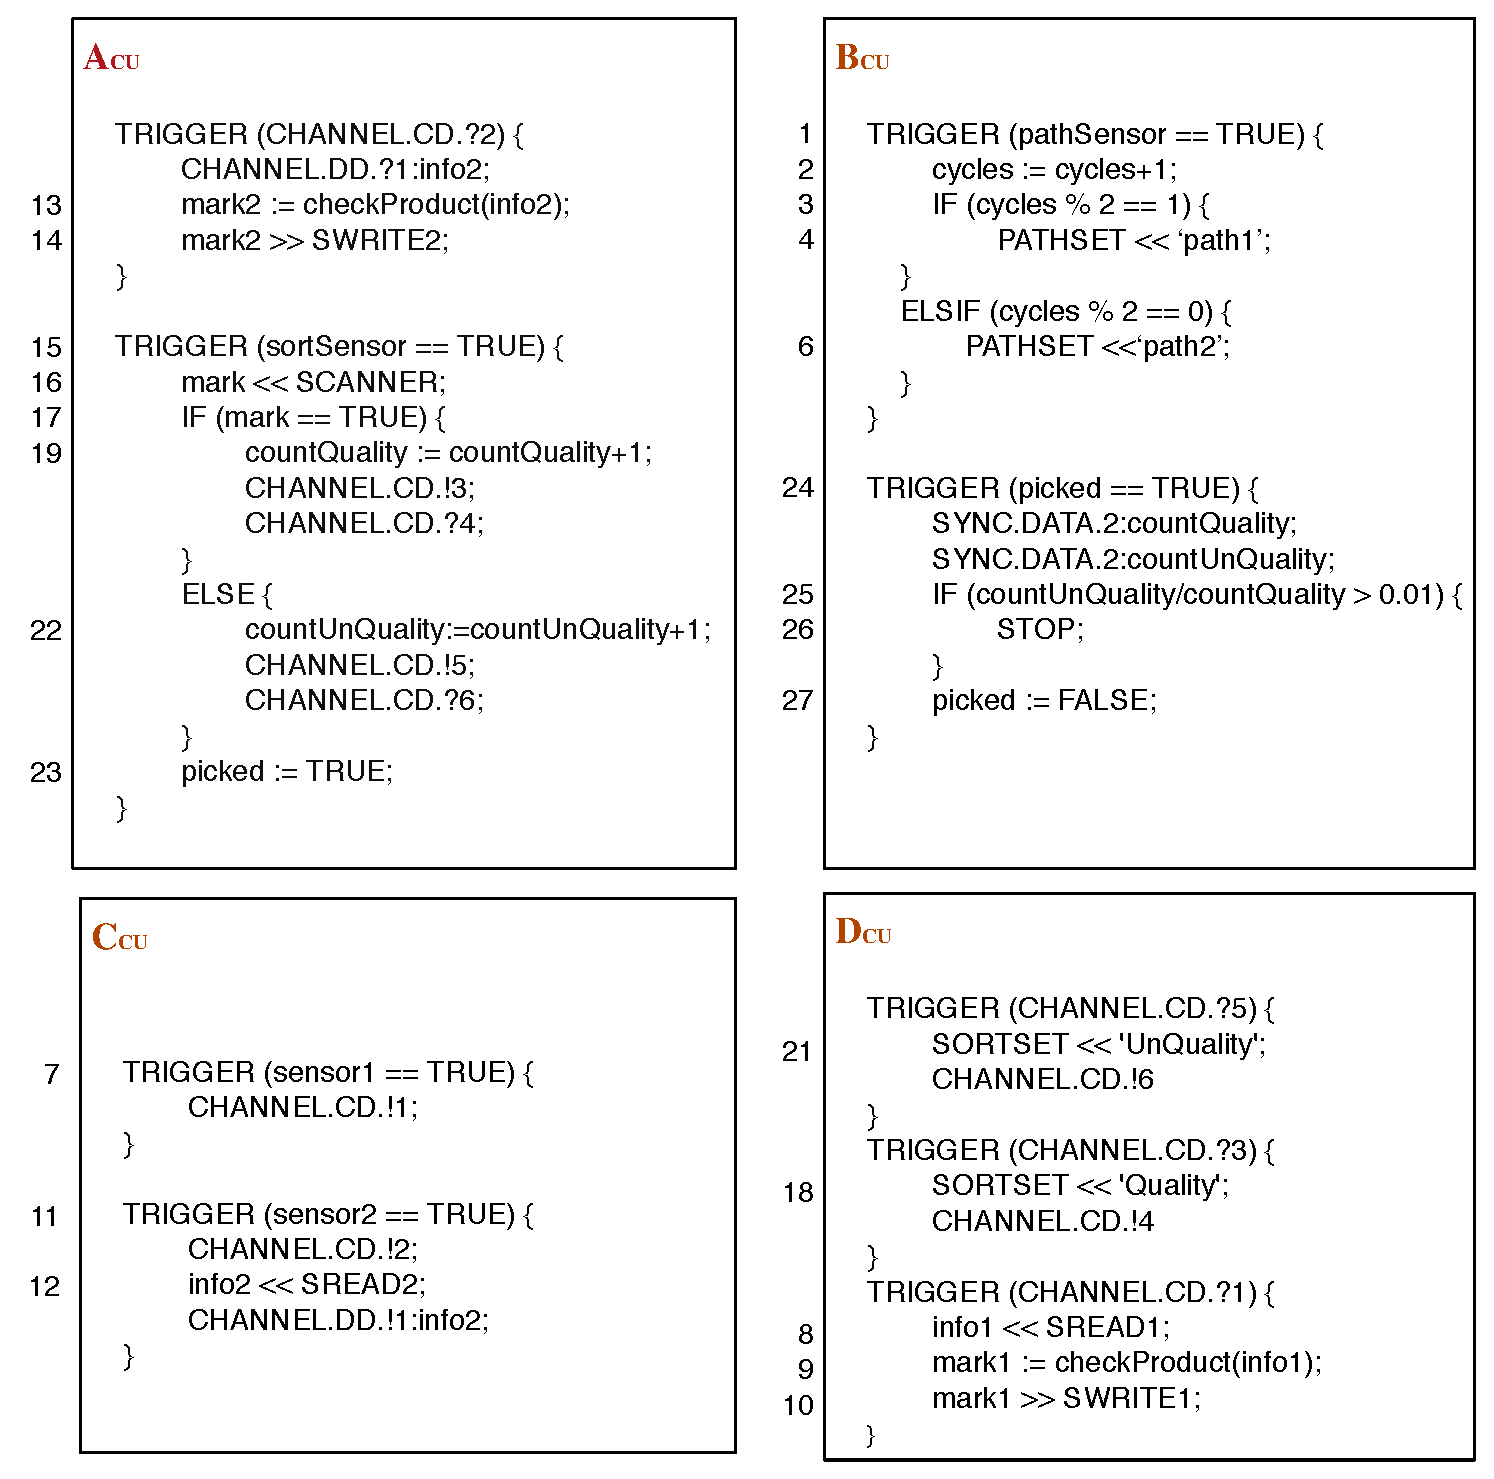
\includegraphics[height=2.4in, width=2.8in]{fig_four_collaborated_program}
    \caption{The collaboration of $A_{cu}$, $B_{cu}$, $C_{cu}$ and $D_{cu}$}\label{fig_four_collaborated_program}
\end{figure}

The implementation of this case study can be cloned from our git repository\footnote{http://code.ntesec.com.cn/ju.li/model-slicing.git}.
